
Auf Basis der in der Balkenberechnung bestimmten Parameter Biegesteifigkeit, maximales Biegemoment und der maximalen Querkraft, sollen die Gurte und der Steg dimensioniert werden. Die Vorauslegung soll dabei anhand der VDI- Richtlinie 2013 erfolgen, diese enthält in einem Unterkapitel Informationen speziell zur Auslegung eines I-Trägers. Dabei ist zu beachten, dass bei einigen Berechnungen Vereinfachungen angenommen werden, die an den betreffenden Stellen spezifiziert werden. Zusätzlich sei angemerkt, dass die erste Auslegung nur an an ausgewählten Stellen Sicherheitsfaktoren ungleich eins berücksichtigt. Grund dafür ist die Annahme, dass in den bereitgestellten Materialkennwerten ausreichende Sicherheiten verrechnet worden sind.

\subsection{Dimensionierung der Gurte zur Einhaltung der Anforderungen an die Steifigkeit}
\begin{figure}
	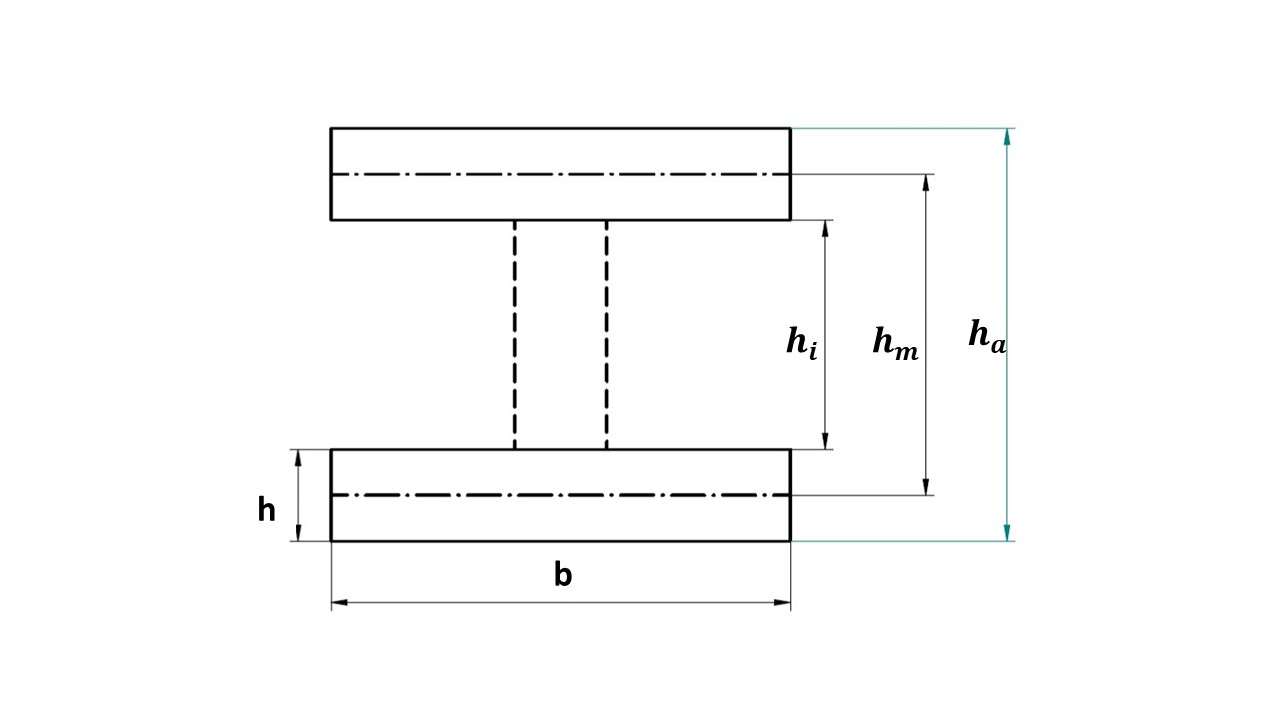
\includegraphics[width=1.0\textwidth]{Bilder/RechteckHolm.jpg}
	\caption{Maße des rechteckigen I-Holms}
	\label{fig: Rechteckholm}
\end{figure}

Bei der Auslegung der Gurte auf Steifigkeit wird angenommen, dass der Steg des I-Trägers keine Längskräfte aufnimmt und der Biegung nicht entgegenwirken kann. Die in der Balkenberechnung ermittelte Biegesteifigkeit $ EI_{x} = 952,55 Nm^{2} $, die erforderlich ist, damit bei einer Kraft $ F_{pruef}=100N $ die Flügelspitze eine Absenkung von $ w_{j=1,1}=20mm $ erfährt, muss allein durch die Gurte aufgebracht werden. Im Sinne der kraftflussgerechten Gestaltung sollen die Glasfasern unidirektional in Längsrichtung des Gurtes angeordnet werden. Die Bezeichnungen der Längenangaben des Holmes orientieren sich an Abb. ~\ref{fig: Rechteckholm}~ .\\



\noindent Die Gurte werden zur Bestimmung der notwendigen Lagenanzahl als rechteckig angenommen, erst in einem späteren Schritt soll die Form der Kontur der vorgegebenen Haut angepasst werden. Die Maße sind über die gesamte Länge des Holms als konstant anzusehen.\\
Zur Bestimmung des Flächenträgheitsmomentes $ I_{x} $ wird der E-Modul in Längsrichtung der Fasern nach der Mischungsregel nach [3] berechnet.\\
\begin{equation}
 E_{11}=  \phi*E_{f,11}+\left( 1-\phi \right) * E_{M}
\end{equation}
Mit den gegebenen Materialkennwerten bestimmt sich $ E_{11} = 31580 MPa $. Damit ergibt sich ein benötigtes Flächenträgheitsmoment von $ I_{x} = 3,01631 * 10^{-8} m^{4} $.
